\documentclass{article}
\usepackage[UTF8]{ctex}
\usepackage[tc]{titlepic}
\usepackage{amsmath, amsthm, amssymb, graphicx}
\usepackage{hyperref}
\usepackage{listings}
\usepackage{titlesec}
\usepackage{cite}
\usepackage{fancyhdr}
\usepackage{booktabs}
\usepackage{graphicx}
\usepackage{geometry}
\usepackage{caption}
\usepackage{subfigure}
\usepackage[section]{placeins}
\geometry{a4paper,scale=0.8}
\pagestyle{fancy}

\lhead{第 4 次作业\\\today}
\chead{中国科学技术大学\\数学建模课程}

\rhead{Assignment 4\\ {\CTEXoptions[today=old]\today}}
\newcommand{\upcite}[1]{\textsuperscript{\cite{#1}}}

\titleformat*{\section}{\bfseries\Large}
\titleformat*{\subsection}{\bfseries\large}

\title{\bfseries 微分方程模型-2019-nCoV传染分析}
\author{Xiaoma \quad   \quad  }

\begin{document}
\maketitle
\begin{abstract}
    本文根据COVID-19与其他传染病的共性,分别基于SI、SIS、SIR、SEIR模型对其进行传染分析。同时根据
    武汉地区疫情初期的确诊以及疑似病例等数据的变化规律对得到的模型进行调整和评估,最终模型的性能和实际传染
    结果基本一致,从而证明了作者的模型与COVID-19的传染模型基本符合。
    
    
\end{abstract}

% \setcounter{secnumdepth}{1}
 \setcounter{section}{1}
\section*{\centerline{一、前言}}
“2019-nCoV”,因2019年武汉病毒性肺炎病例而被发现,2020年1月12日被世界卫生组织命名,已经肆虐全球三年多,很多国家反复多次,
虽然目前病毒的毒性已经大大减弱,但其仍对日常生活有较大的影响,所以对其建立传染模型进行分析以及预测疫情的后续发展是
至关重要的。


 \setcounter{section}{2}
\section*{\centerline{二、相关工作}}
\begin{enumerate}
    \item 建立基本的SI、SIS、SIR、SEIR模型
    \item 根据实际数据进行参数调整
    \item 对未来疫情发展进行预测,以及对影响疫情发展的相关因素的分析
\end{enumerate}

 \setcounter{section}{3}
\section*{\centerline{三、问题分析}}
    目前国内已经对主流的新冠病毒毒株产生群体免疫,故若有下一轮疫情爆发很可能是因为变异新毒株,故
    使用疫情初期武汉的确诊以及疑似病例等数据来进行分析,更符合对未来预测的准确性。
    \begin{figure*}[htbp]
        \centering
        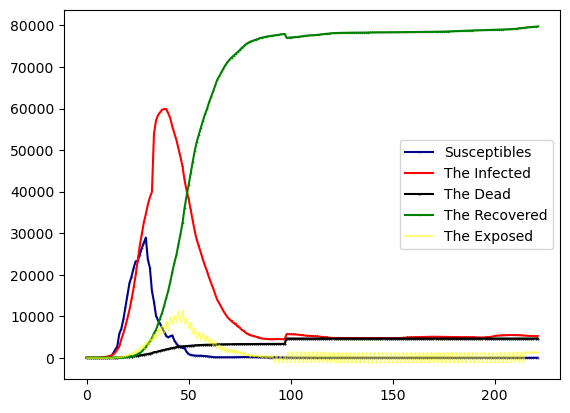
\includegraphics[width=0.8\textwidth]{./img/0.png}
        \caption*{\text{实际数据}}
    
    \end{figure*}
\section*{\centerline{四、建模的假设}}
    \subsection{假设1}
    假设疫情初期只有一种病毒毒株
    \subsection{假设2}
    假设在数据统计期间该地区无大规模人口流动

\clearpage

 \setcounter{section}{5}
 \section*{\centerline{五、符号说明}}
 \begin{table}[htbp]
    
    \centering%把表居中
    \begin{tabular}{cc}%内容全部居中
    \toprule%第一道横线
    符号&说明 \\
    S(Susceptibles) & 可能被感染者\\
    E(Exposed) & 潜伏者\\
    I(Infected) & 感染者\\
    R(Recovered) & 康复者\\
    D(Dead) & 死亡者\\
    $\beta$ & 病毒传染给健康者的概率\\
    $\gamma_{1}$& 潜伏期治愈率\\
    $\gamma_{2}$&感染者治愈率\\
    $\alpha$& 潜伏者转换为感染者的比例\\
    $\theta$& 死亡率\\

    \bottomrule%第三道横线
    \end{tabular}
\end{table}

 \setcounter{section}{6}
\section*{\centerline{六、数学模型建立}}
\subsection*{SI模型}
SI模型是一种传染病模型,适用于只有易感者和患病者两类人群,且不会反复发作的疾病。
模型假设易感者与患病者有效接触即被感染,变为患病者,无潜伏期、无治愈情况、无免疫力。
以一天作为模型的最小时间单元。总人数为N,不考虑人口的出生与死亡,迁入与迁出,此总人数不变。
t时刻两类人群占总人数的比率分别记为$s(t)$、$i(t)$,两类人群的数量为$S(t)$、$I(t)$。
初始时刻$t=0$时,各类人数量所占初始比率为$s0$、$i0$。
每个患病者每天有效接触的易感者的平均人数是$\lambda$,即日接触数。
根据模型假设,每天可使$\lambda s(t)$个易感者变为患病者,且患病者人数为$Ni(t)$,
所以每天有$\lambda s(t)Ni(t)$个易感者被感染,即每天新增的患病者数,
可得微分方程:$$Ndi(t)/dt=\lambda s(t)Ni(t)$$因为$s(t)+i(t)=1$,
故可得SI模型为:$$\begin{cases}
    di(t)/dt=\lambda (1-i(t))i(t)\\
    i(0)=i0
\end{cases}$$
运用Logistic模型解得$$i(t)=1/(1+(1/i0-1)exp(-\lambda t))$$
患病人数$I(t)=Ni(t)1$。

\subsubsection*{SI模型结果}
\begin{figure*}[htbp]
    \centering
	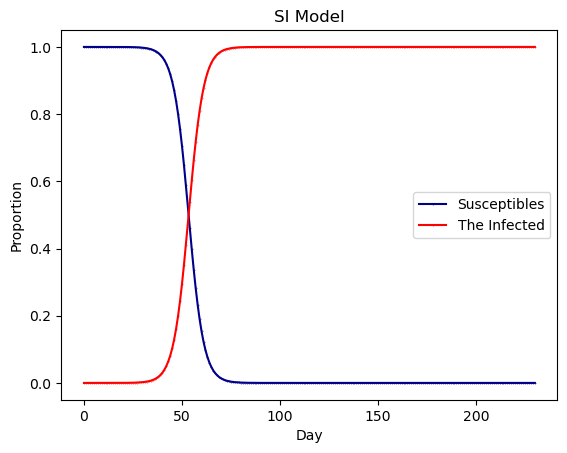
\includegraphics[width=0.8\textwidth]{./img/1.png}
    \caption*{\text{SI模型}}

\end{figure*}

根据结果可知该模型无法模拟实际数据。
\subsection*{SIS模型}
SIS模型是一种传染病模型,适用于只有易感者和患病者两类人群,
且会反复发作的疾病。模型假设易感者与患病者有效接触即被感染,
变为患病者,无潜伏期、无治愈情况、无免疫力。
以一天作为模型的最小时间单元。总人数为N,
不考虑人口的出生与死亡,迁入与迁出,此总人数不变。
t时刻两类人群占总人数的比率分别记为$s(t)$、$i(t)$,
两类人群的数量为$S(t)$、$I(t)$。初始时刻t=0时,
各类人数量所占初始比率为$s0$、$i0$。
每个患病者每天有效接触的易感者的平均人数是$\lambda$,
即日接触数。根据模型假设,每天可使$\lambda s(t)$个易感者变为患病者,
且患病者人数为$Ni(t)$,所以每天有$\lambda s(t)Ni(t)$个易感者被感染,
即每天新增的患病者数,
可得微分方程:$$Ndi(t)/dt=\lambda s(t)Ni(t)-\mu Ni(t)$$
因为$s(t)+i(t)=1$
故可得SIS模型为:$$\begin{cases}
    di(t)/dt=\lambda (1-i(t))i(t)-\mu i(t)\\
    i(0)=i0
\end{cases}$$
运用Logistic模型解得$$i(t)=\lambda /(\mu +\lambda e^(-\lambda t))$$患病人数$$I(t)=N*i(t)1$$

\subsubsection*{SIS模型结果}
\begin{figure*}[htbp]
    \centering
	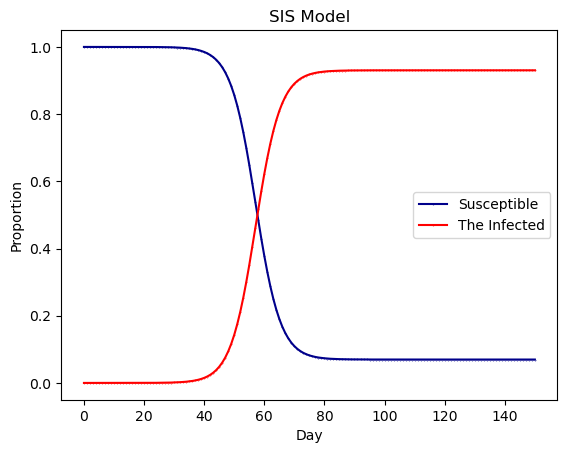
\includegraphics[width=0.8\textwidth]{./img/2.png}
    \caption*{\text{SI模型}}

\end{figure*}

根据后续对新冠病毒的研究可知,正常情况下不会二次感染同种毒株,则该模型同样不能模拟实际数据。

\subsection*{SIR模型}
SIR模型是一种传染病模型,适用于有易感者、患病者和康复者三类人群,治愈后不会再发的疾病。
模型假设易感者与患病者有效接触即被感染,变为患病者,可被治愈变为康复者,无潜伏期,有终身免疫力。
以一天作为模型的最小时间单元。
总人数为N,不考虑人口的出生与死亡,迁入与迁出,此总人数不变。
t时刻各类人群占总人数的比率分别记为$s(t),i(t),r(t)$,各类人群的数量为$S(t),I(t),R(t)$。
初始时刻$t=0$时,各类人数量所占初始比率为$s0,i0,r0$。
日接触数$\lambda$,即每个患病者每天有效接触的易感者的平均人数。
日治愈率$\mu$,即每天被治愈的患病者人数占病人总数的比率。
根据模型假设,每个病人每天可使$\lambda s(t)$个易感者变为患病者,
且患病者人数为$Ni(t)$,所以每天有$\lambda s(t)Ni(t)$个易感者被感染,
即每天新增的患病者数。每天的患病人数$Ni(t)$中,
又有$\mu Ni(t)$被治愈成为康复者。
可得微分方程:
$$\begin{cases}
    Nds(t)/dt=-\lambda s(t)Ni(t)\\
    Ndi(t)/dt=\lambda s(t)Ni(t)-\mu Ni(t)\\
    Ndr(t)/dt=\mu Ni(t)
\end{cases}$$

同约N后得:
$$ds(t)/dt=-\lambda s(t)i(t)$$
$$di(t)/dt=\lambda s(t)i(t)-\mu i(t)$$
$$dr(t)/dt=\mu *i(t)$$
$$s(0)=s0,i(0)=i0,r(0)=r0$$

此模型无解析解,给定$\lambda ,\mu ,s0,i0$可求数值解。
\subsubsection*{SIR模型结果}

\begin{figure}[h!]
    \centering
        \subfigure[$\text{0天为起始预测}$]{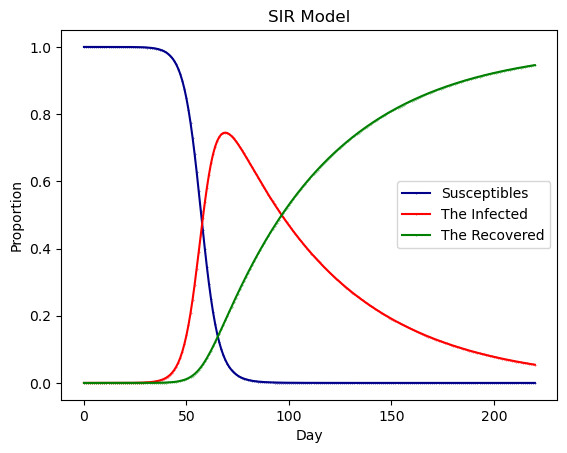
\includegraphics[width=0.4\hsize]{./img/4.png}}  
        \subfigure[$\text{30天为起始预测}$]{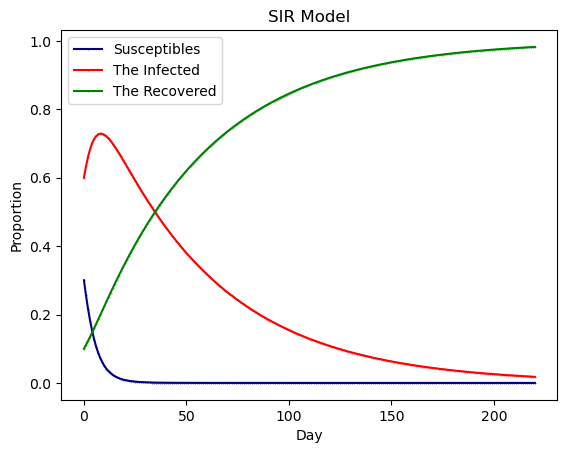
\includegraphics[width=0.4\hsize]{./img/3.png}} 
        
\end{figure}

由图可知,得到的结果与实际数据已经十分相似,但仍有部分预测与实际不符,考虑到
武汉后期封城,在中期变更确诊标准(临床观察结果与核酸检测等效),后期居民的防护意识以及医院的治疗
方法的提高等原因,对该模型的参数进行一定的修改。

\begin{enumerate}
    \item 变更确诊标准导致实际数据在确诊数量的峰值附近增长更快,但此时多出的确诊数量可能是在之前就已经被感染的患者,
    故实际数据在前期会有一定误差,而我们的SIR模型可能更精确,故此原因不做调整。
    \item 封城、易感染者提高防护意识、医疗水平提高会导致后期的感染率下降,故使用时间衰减的方式降低感染率,提高疾病治愈率。
\end{enumerate}
\clearpage
\subsubsection*{调整后的SIR模型结果}
\begin{figure}[h!]
    \centering
        \subfigure[$\text{0天为起始预测}$]{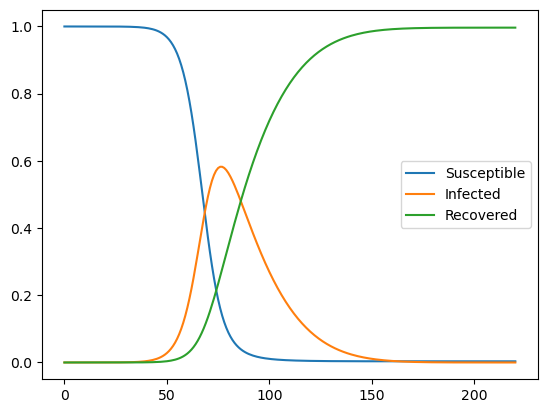
\includegraphics[width=0.4\hsize]{./img/6.png}}  
        \subfigure[$\text{30天为起始预测}$]{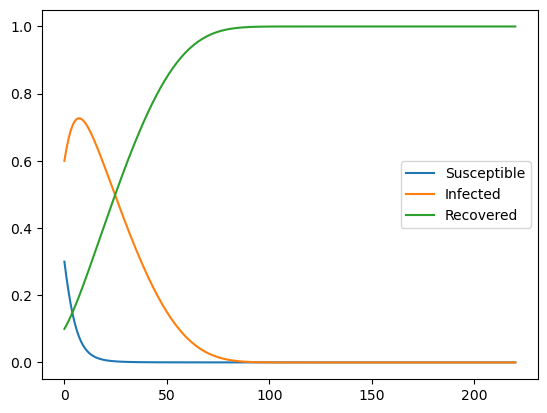
\includegraphics[width=0.4\hsize]{./img/5.png}} 
        
\end{figure}

由图可知模型的拟合程度得到了进一步的提高,但新冠病毒携带者常常伴随着潜伏期,这是SIR模型无法
考虑的。

\subsection*{SEIR模型}
SEIR模型是一种常用的传染病模型,它将人群分为四类:
易感者(Susceptible)、潜伏者(Exposed)、
感染者(Infected)和康复者(Recovered)。
模型中每个类别的人数随时间变化的动态可以用以下微分方程组来描述:
$$\begin{cases}
    \frac{d S}{d t} & =-\frac{\beta S I}{N} \\
\frac{d E}{d t} & =\frac{\beta S I}{N}-\sigma E \\
\frac{d I}{d t} & =\sigma E-\gamma I \\
\frac{d R}{d t} & =\gamma I
\end{cases}$$
其中,$S$表示易感者人数,
$E$表示潜伏者人数,$I$表示感染者人数,
$R$表示康复者人数,$N=S+E+I+R$表示总人数。
$\beta$表示传染率,即每个单位时间内,
一个感染者能够感染的易感者人数。
$\sigma$表示潜伏者转变为感染者的速率。
$\gamma$表示康复率,即每个单位时间内,
有多少感染者康复。
\clearpage
\subsubsection*{SEIR模型结果}

\begin{figure}[h!]
    \centering
        \subfigure[$\text{0天为起始预测}$]{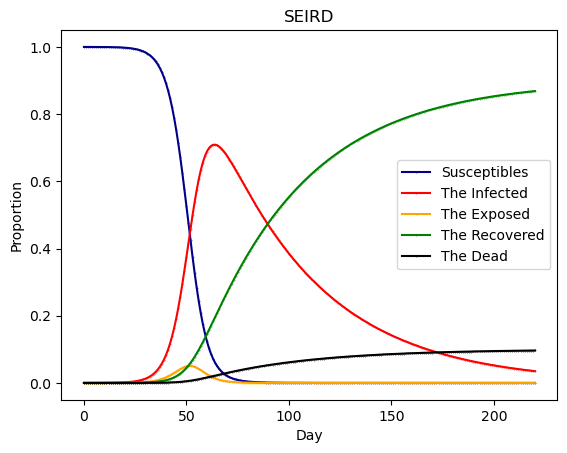
\includegraphics[width=0.4\hsize]{./img/9.png}}  
        \subfigure[$\text{30天为起始预测}$]{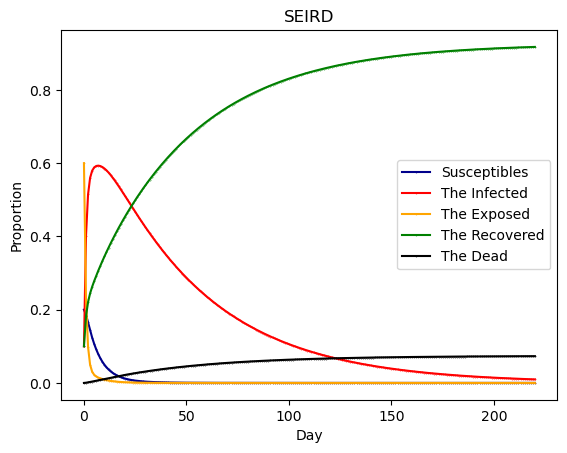
\includegraphics[width=0.4\hsize]{./img/10.png}} 
        
\end{figure}

继续考虑封城等其他因素
\subsubsection*{调整后的SEIR模型结果}
\begin{figure}[h!]
    \centering
        \subfigure[$\text{0天为起始预测}$]{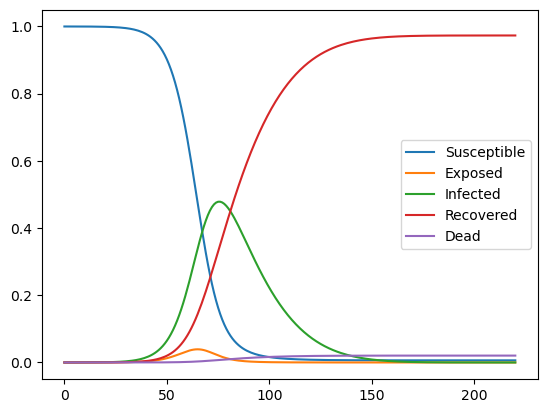
\includegraphics[width=0.4\hsize]{./img/7.png}}  
        \subfigure[$\text{30天为起始预测}$]{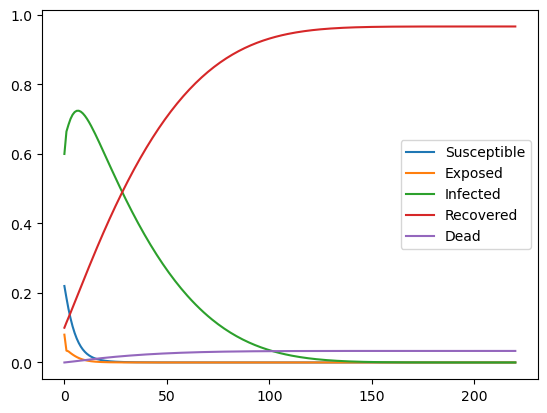
\includegraphics[width=0.4\hsize]{./img/8.png}} 
        
\end{figure}

由图可知,该模型可以较好的模拟实际数据。

\section*{\centerline{八、结论}}
\begin{enumerate}
    \item 对未来的预测:目前国内的疫情趋势已经达到模型中的后部分,即已产生
    群体免疫,但若有新毒株出现时,疫情趋势可能与模型的前半部分更相近。
    \item 在与新冠病毒共存的过程中,应从降低暴露率,降低感染率等方面入手,
    增强防护的意识以及增强身体素质。
\end{enumerate}
 \setcounter{section}{9}
\section*{\centerline{九、问题}}
    \begin{enumerate}
        \item 考虑到使用全国的数据量过大,以及疫情放开后的数据不够准确等原因,仅使用了武汉地区的数据,泛化性可能较差。
        \item 未考虑次密接者的数据。
    \end{enumerate}
 
\bibliographystyle{plain}
\bibliography{refer}
\end{document}